\documentclass[green]{beamer}

\usepackage[utf8]{inputenc}
\usepackage[spanish,activeacute]{babel}
\usepackage{graphicx} % Imágenes
\usepackage{fancyhdr} % Cabeceras
\usepackage{listings}
\usepackage{licencia}

\definecolor{verde}{rgb}{0.4,0.6,0.2}
\definecolor{verdeunix}{rgb}{0.05,0.5,0.05}
\definecolor{verde2}{rgb}{0.2,0.5,0.2}

\usefonttheme{structuresmallcapsserif} 
\useoutertheme{shadow} 
\usetheme{Frankfurt}
\useinnertheme{rounded}
\setbeamercovered{transparent}

%\usetheme{Berlin}
\usecolortheme[named=verdeunix]{structure}

\title[IberOgre y Sion Tower]{IberOgre, wiki sobre Ogre3D y\\Sion Tower, videojuego de estrategia}
\author[David Saltares Márquez]{Ingeniería Técnica en Informática de Gestión\\David Saltares Márquez}
\date{Septiembre de 2011}

\AtBeginSection[]
{
    \begin{frame}<beamer>
    \transdissolve
        \frametitle{Índice}
        \tableofcontents[currentsection,currentsubsection]
    \end{frame}
}

\begin{document}

\begin{frame}[fragile]
\transdissolve
    \titlepage 
	
    \begin{picture}(0,0)
        \put(10,-5){
\includegraphics[scale=0.2]{img/personaje.png}}
    \end{picture}
    
    \begin{picture}(0,0)
        \put(230,25){
\includegraphics[scale=0.06]{img/iberogre.png}}
    \end{picture}
	
    {\scriptsize
	\begin{center}
	    \begin{verbatim}
	             https://forja.rediris.es/projects/cusl5-iberogre
	    \end{verbatim}
	\end{center}
    }
    
    \begin{picture}(0,0)
        \put(135,10){
\includegraphics[scale=0.4]{img/cc-by-nc-sa.png}}
    \end{picture}
\end{frame}

\begin{frame}[fragile]
\transdissolve
    \frametitle{Índice}
    \tableofcontents
\end{frame}


% Introducción
\section{Introducción}

% Proyecto propuesto

\begin{frame}{Proyecto propuesto}
    \begin{columns}[t]
    
    \column{150px}
	\begin{center}
	    
\includegraphics[scale=0.1]{img/iberogre.png}
	\end{center}
	\begin{block}{IberOgre}
	    Wiki sobre desarrollo de videojuegos en 3D
	    con \textsc{Ogre3D}.
	\end{block}
	
    \column{150px}
	\begin{center}
	    
\includegraphics[scale=0.18]{img/personaje.png}
	\end{center}
	\begin{block}{SionTower}
	    Videojuego de estrategia y acción con \textsc{Ogre3D}.
	\end{block}
    
    \end{columns}
\end{frame}


% Ogre3D

\begin{frame}{¿Qué es Ogre?}    
    \begin{center}
	\emph{\textbf{\huge{O}}bject Oriented \textbf{\huge{G}}raphics \textbf{\huge{R}}endering \textbf{\huge{E}}ngine}
    \end{center}

    \begin{columns}[t]
    \column{150pt}
	\begin{block}{Ofrece}
            \begin{itemize}
                \item Abstracción de OpenGL y DirectX.
		\item Libre (MIT)
                \item Motor profesional
                \item Extensible y configurable.
            \end{itemize}            
        \end{block}

    \column{150pt}
	\begin{alertblock}{No ofrece}
            \begin{itemize}
                \item Colisiones.
		\item Audio.
                \item Entrada de usuario.
                \item Red.
            \end{itemize}            
        \end{alertblock}
    \end{columns} 
    
\end{frame}

\begin{frame}
    \frametitle{Utilizado en juegos libres...}
    
    \begin{center}
	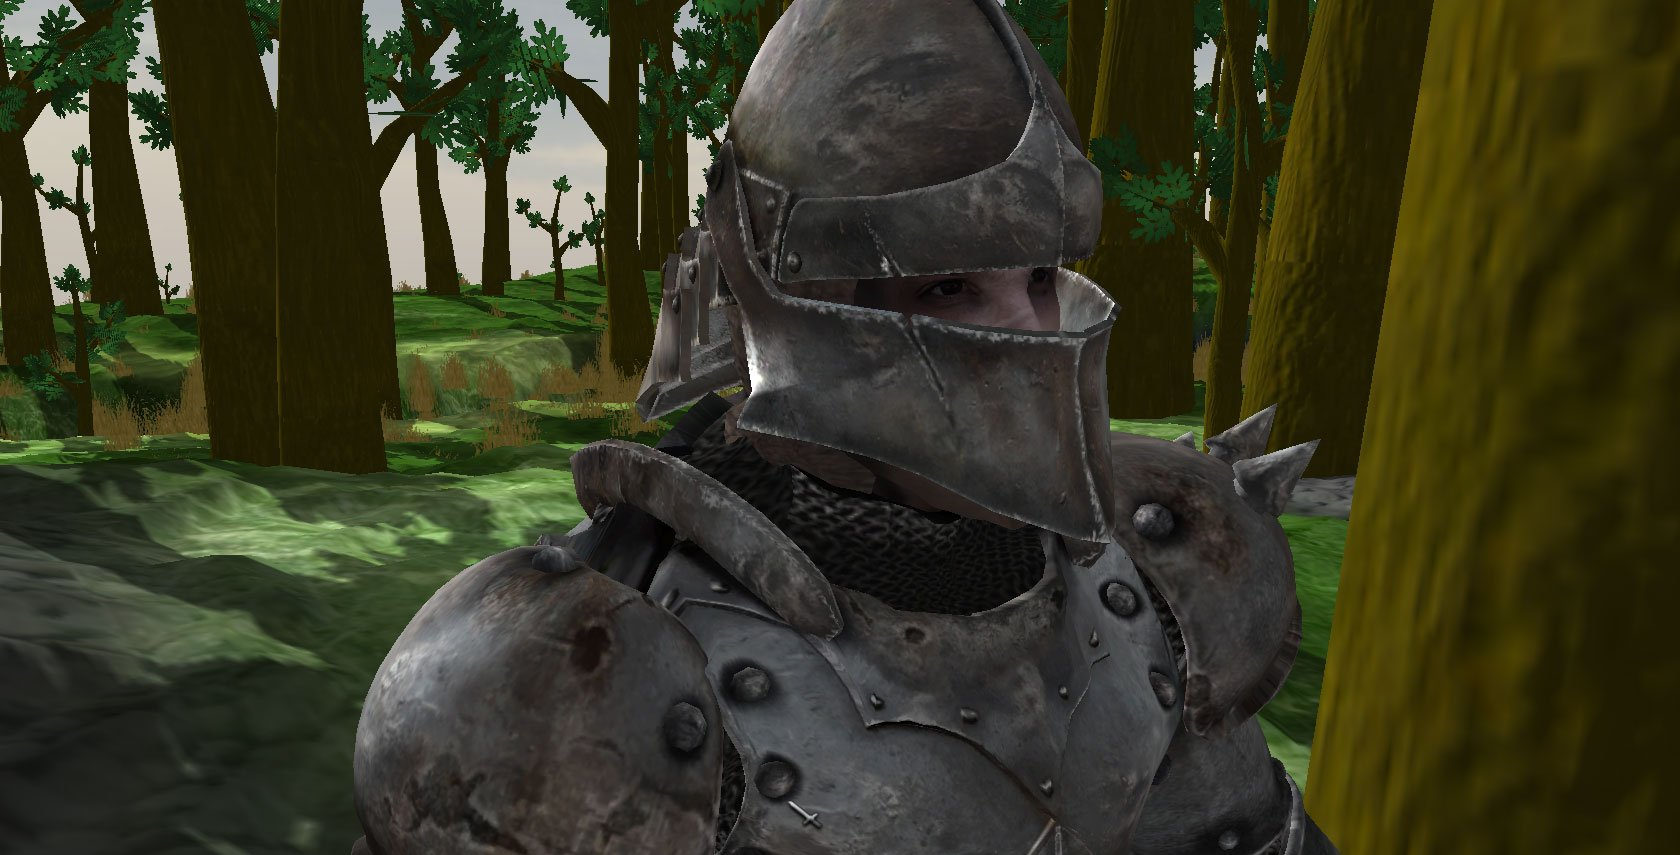
\includegraphics[scale=0.18]{img/abaddon.jpg}
	    
	\tiny{Abaddon}
    \end{center}
\end{frame}

\begin{frame}
    \frametitle{Utilizado en juegos libres...}
    
    \begin{center}
	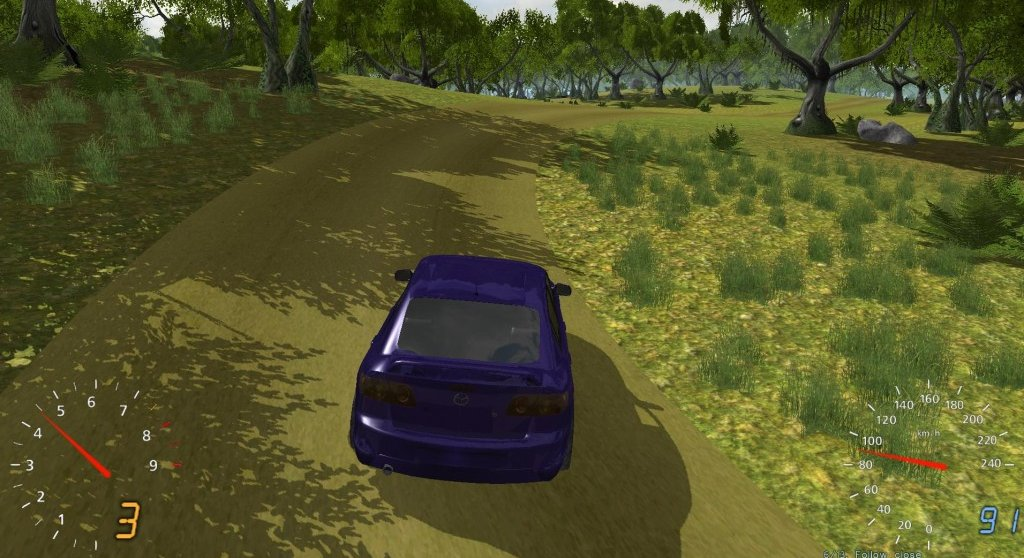
\includegraphics[scale=0.25]{img/stuntrally.jpg}
	    
	\tiny{Stunt Rally}
    \end{center}
\end{frame}

\begin{frame}
    \frametitle{... Y también en juegos comerciales}
    
    \begin{center}
	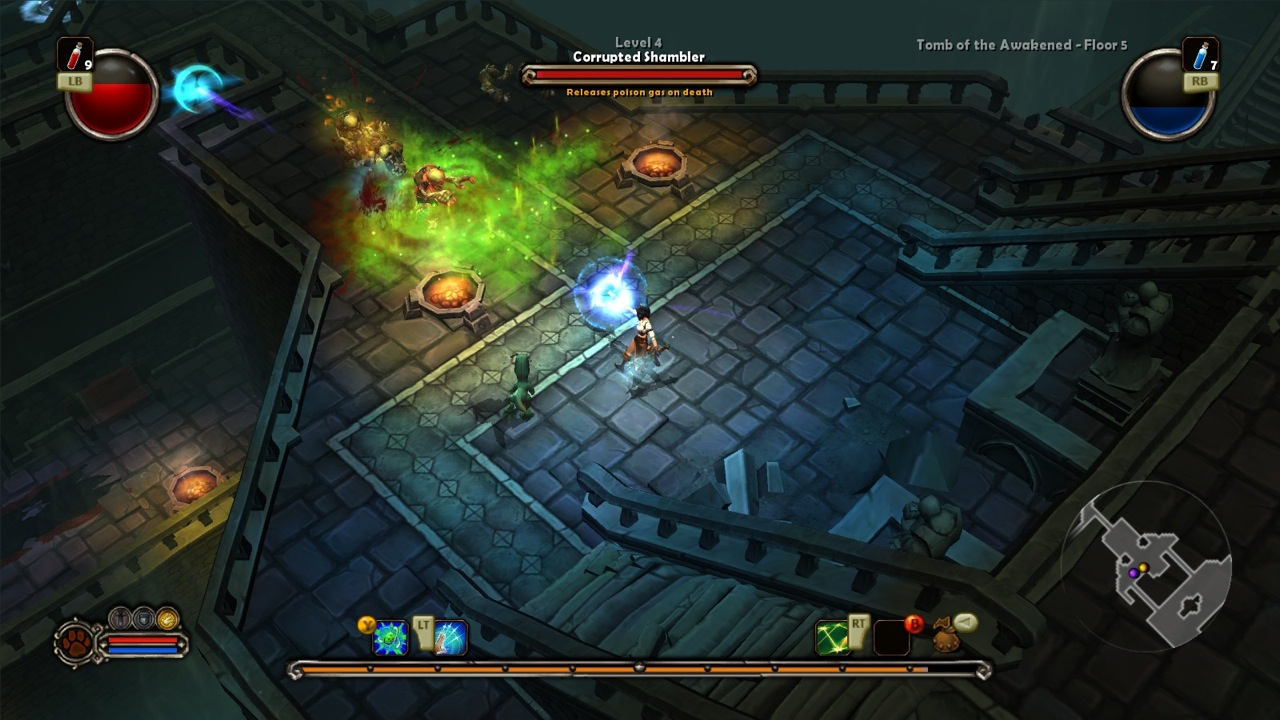
\includegraphics[scale=0.22]{img/torchlight.jpg}
	    
	\tiny{Torchlight (Runic Games - Windows, Mac OS X, Xbox 360 - 2009)}
    \end{center}
\end{frame}

\begin{frame}
    \frametitle{... Y también en juegos comerciales}
    \begin{center}
	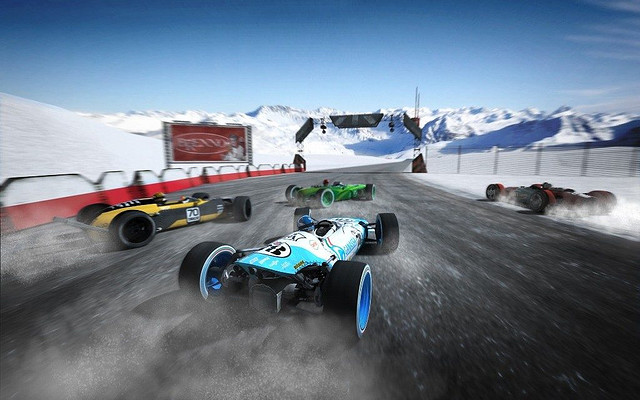
\includegraphics[scale=0.4]{img/victory.jpg}
	    
	\tiny{Victory: Age of Racing (GamersFirst - Windows - 2011)}
    \end{center}
\end{frame}

% Motivaciones

\begin{frame}{Motivaciones}
    \begin{columns}[t]
    
    \column{150px}
	\begin{block}{IberOgre}
	    \begin{itemize}
		\item Ausencia de documentación en castellano.
		\item Aunar motor y base matemática.
		\item Ampliación Diseño de Videojuegos.
		\item ADVUCA
	    \end{itemize}
	\end{block}
	
    \column{150px}
	\begin{block}{SionTower}
	    \begin{itemize}
		\item Aprender a desarrollar videojuegos 3D.
		\item \textsc{Ogre3D} es profesional.
		\item Futuro laboral.
	    \end{itemize}
	\end{block}
    
    \end{columns}
\end{frame}

% Objetivos

\begin{frame}{Objetivos}
    \begin{columns}[t]
    
    \column{200px}
	\begin{block}{IberOgre}
	    \begin{itemize}
		\item Subsistemas de \textsc{Ogre3D}.
		\item Conocimientos matemáticos mínimos.
		\item Tecnologías complementarias.
		\item Aproximación práctica.
		\item Herramientas libres y multiplataforma.
		\item Buenas prácticas.
		\item Construir una comunidad.
	    \end{itemize}
	\end{block}
	
    \column{100px}
    
    \begin{center}
	
\includegraphics[scale=0.22]{img/sinbad.png}
    \end{center}
    
    \end{columns}
\end{frame}

\begin{frame}{Objetivos}
    \begin{columns}[t]
    
    \column{200px}
	\begin{block}{Sion Tower}
	    \begin{itemize}
		\item Ejemplo \textbf{real} de videojuego.
		\item Creación de niveles.
		\item Trabajo en equipo.
		\item Diversión.
		\item Subsistemas reutilizables.
	    \end{itemize}
	\end{block}
	
    \column{100px}
    
    \begin{center}
	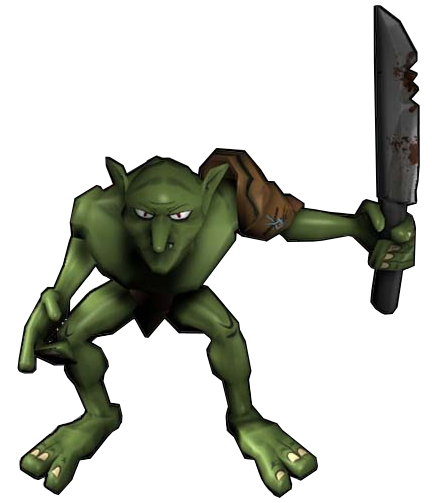
\includegraphics[scale=0.23]{img/goblin.png}
    \end{center}
    
    \end{columns}
\end{frame}

% Calendario
\section{Calendario}

\begin{frame}{Diagrama de Gantt (1/2)}
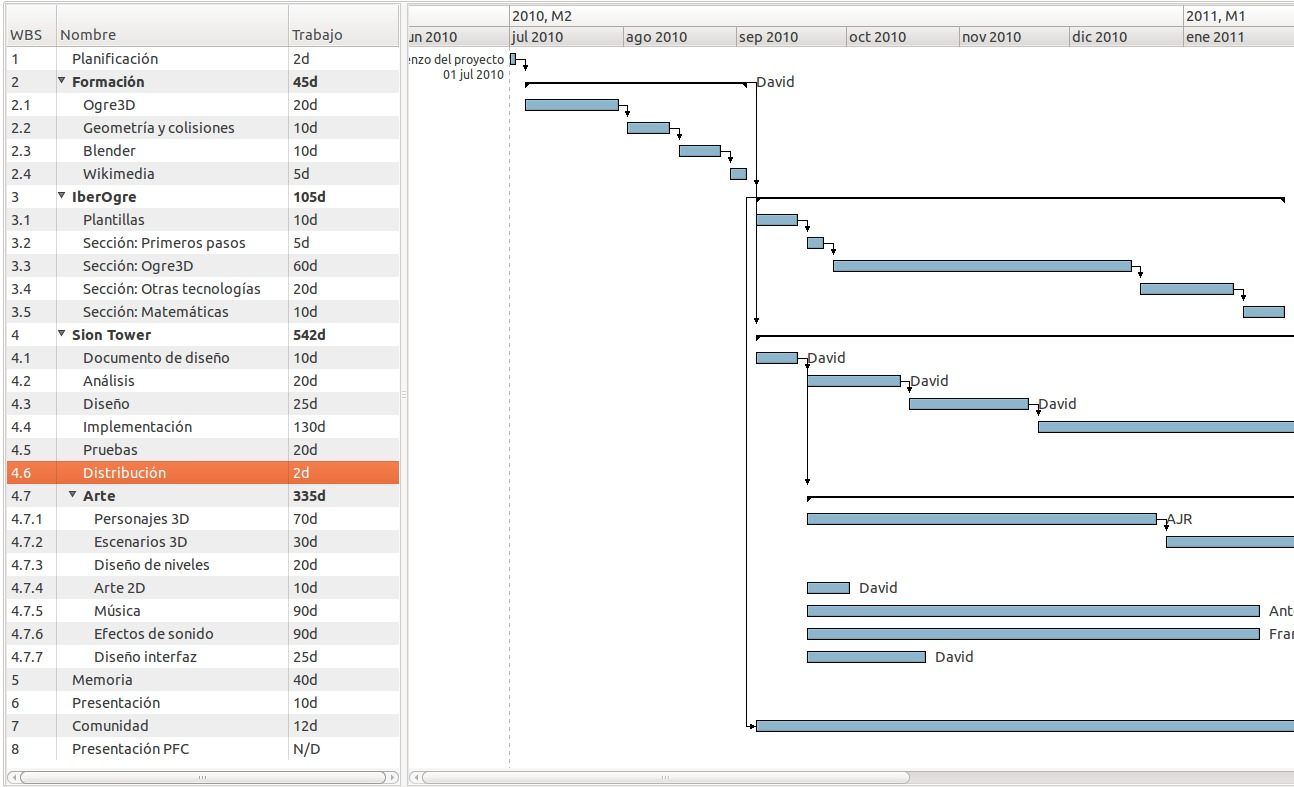
\includegraphics[scale=0.24]{img/planificacion1.jpg}
\end{frame}

\begin{frame}{Diagrama de Gantt (2/2)}
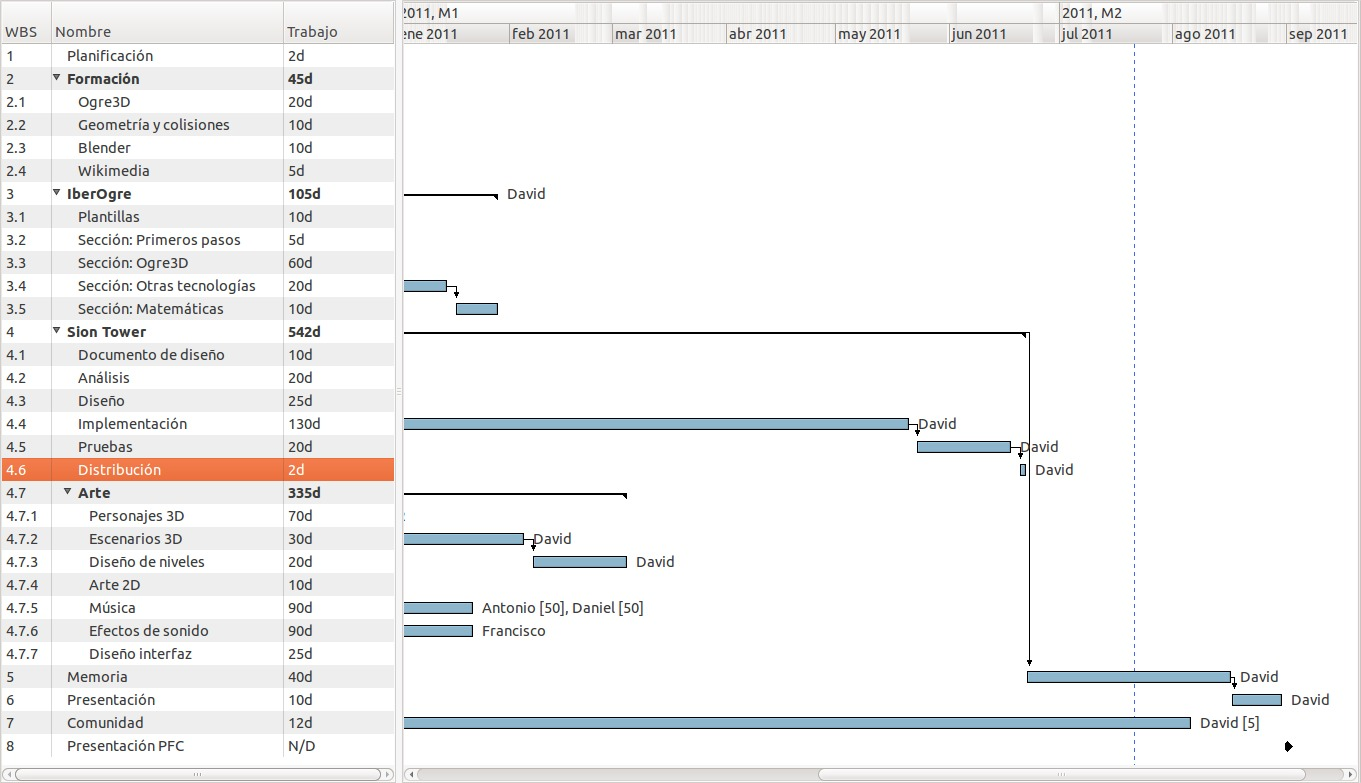
\includegraphics[scale=0.24]{img/planificacion2.jpg}
\end{frame}

% Desarrollo IberOgre
\section[IberOgre]{Desarrollo de IberOgre}

    % Metodología
    
\begin{frame}{Metodología}
    
    IberOgre es un proyecto software, \textit{RUP} difícil de aplicar.
    
    \begin{block}{Metodología seguida}
	\begin{enumerate}
	    \item Estudio de necesidades.
	    \item Planificación.
	    \item Redacción y formateado.
	    \item Desarrollo del ejemplo.
	    \item Evaluación.
	\end{enumerate}
    \end{block}
    
    Se utiliza el motor MediaWiki.
    
\end{frame}

    % Estructura de artículos
    
\begin{frame}{Estructura de los artículos}
    
    \begin{center}
	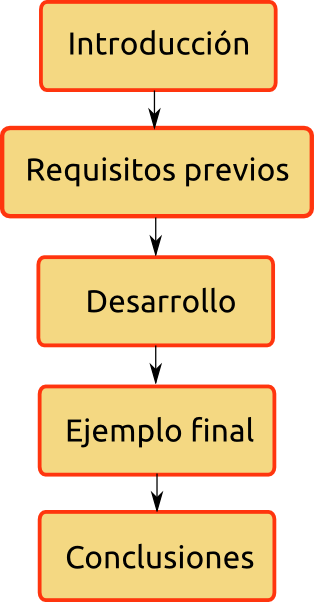
\includegraphics[scale=0.5]{img/bloques-articulos.png}
    \end{center}

\end{frame}
    
    % Artículos
    
\begin{frame}
    \frametitle{Artículos}
        
    \begin{columns}[c]
    \column{180pt}
        
	\begin{block}{Secciones}
            \begin{itemize}
                \item Programación de videojuegos 3D
		\item Ogre3D
		\item Otras tecnologías
		\item Videojuegos
            \end{itemize}            
        \end{block}
	
    \column{60pt}
        
	\begin{center}
	    
\includegraphics[scale=0.55]{img/iberogre-cabeza.png}
	\end{center}
	
	\begin{center}
	    
\includegraphics[scale=0.18]{img/vectores.png}
	\end{center}

	\begin{center}
	    
\includegraphics[scale=0.25]{img/tux.png}
	\end{center}
	
    \column{60pt}
	
	\begin{center}
	    
\includegraphics[scale=0.45]{img/particulas.png}
	\end{center}
	
	\begin{center}
	    
\includegraphics[scale=0.5]{img/joystick.png}
	\end{center}
	
	\begin{center}
	    
\includegraphics[scale=0.5]{img/pintura.png}
	\end{center}
	
    \end{columns} 
\end{frame}
    
    
    % Ejemplos

\begin{frame}{Ejemplos}
    
    \begin{center}
	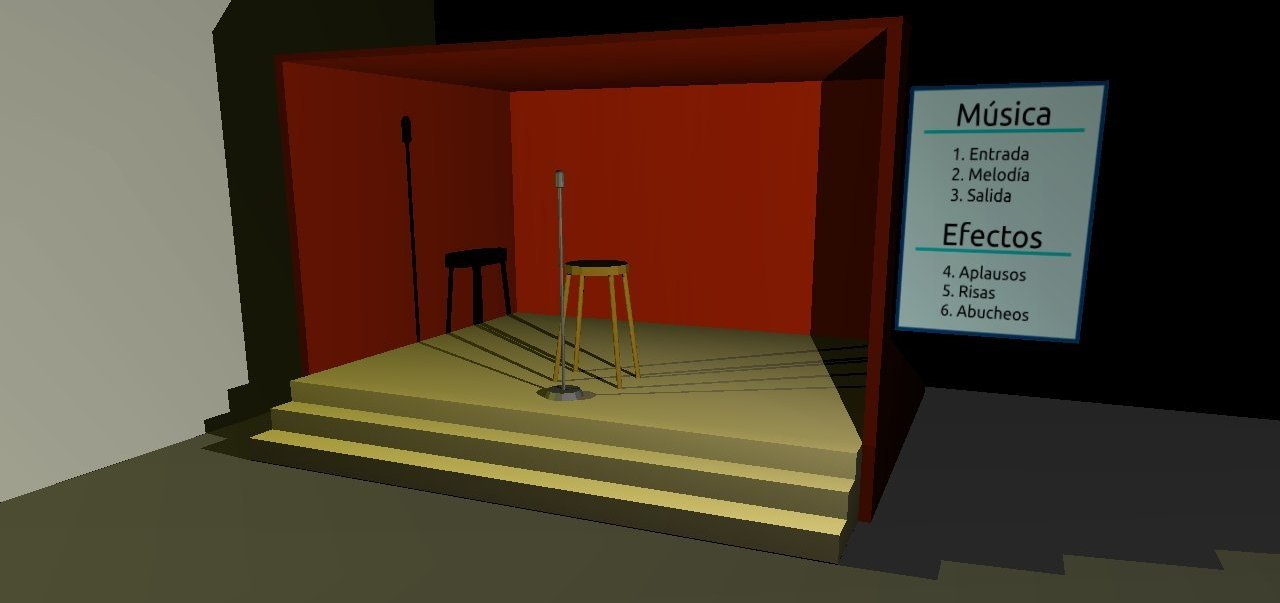
\includegraphics[scale=0.22]{img/ejemplo-audio.jpg}
    \end{center}
    
    \begin{block}{Características}
	\begin{itemize}
	    \item Resumen el artículo de forma práctica.
	    \item Esquema común.
	    \item Completamente documentados.
	\end{itemize}
    \end{block}
    
\end{frame}


    

% Desarrollo Sion Tower
\section[Sion Tower]{Desarrollo de Sion Tower}

    % Equipo de desarrollo
    
\begin{frame}{Equipo de desarrollo}
    
    \begin{center}
	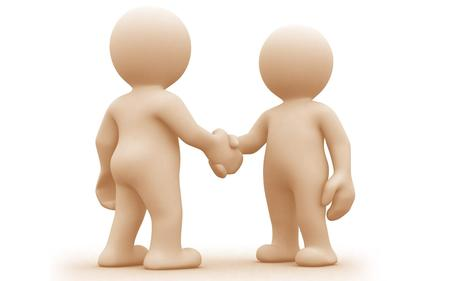
\includegraphics[scale=0.12]{img/colaboradores.jpg}
    \end{center}
    
    Equipo multidisciplinar, metodología RUP, notación UML.
    
    \begin{block}{Miembros}
	\begin{itemize}
	    \item Antonio Jiménez Rodríguez: arte 3D.
	    \item Daniel Pellicer García y Antonio Caro Oca: BSO.
	    \item Francisco Martín Márquez: efectos de sonido.
	    \item Daniel Belohlavek: iconos 2D.
	    \item Varios: testeo.
	\end{itemize}
    \end{block}
    
    Solucionar problemas de coordinación y formato de entregas.
    
\end{frame}

    % Documento de diseño
    
\begin{frame}{Documento de diseño}

    
    En primer lugar se elaboró el documento de diseño del juego.

    \begin{columns}[t]
    \column{150pt}
        
	\begin{block}{Contiene}
            \begin{itemize}
                \item Descripción del juego.
		\item Mecánicas.
		\item Personajes, objetos y habilidades.
		\item Interfaz.
		\item Lista de recursos.
            \end{itemize}            
        \end{block}

    \column{150pt}
        
	\begin{block}{Me ayudó a}
            \begin{itemize}
                \item Dejar por escrito lo que iba a desarrollar.
		\item Conseguir colaboradores.
		\item Misma concepción del juego.
            \end{itemize}            
        \end{block}
    \end{columns} 
    
\end{frame}
    
    % Internacionalización mediante gettext
    
\begin{frame}{Internacionalización mediante gettext}
    
    \textsc{gettext} es una biblioteca libre muy utilizada de i18n.
    
    \begin{alertblock}{Problema}
	\begin{itemize}
	    \item Obtener plantillas de traducción.
	    \item Algunas cadenas están en el código.
	    \item Algunas cadenas están en plantillas de interfaz XML.
	\end{itemize}
    \end{alertblock}
    
    \begin{block}{Solución}
	Script en \textit{Python} para extraer cadenas.
    \end{block}
    
\end{frame}
    
    % Sistema de audio 3D

\begin{frame}{Sistema de audio}
    
    \begin{alertblock}{Problema}
	\begin{itemize}
	    \item \textsc{Ogre3D} no incluye subsistema de audio.
	    \item Necesidad de utilizar una biblioteca externa.
	    \item Integración del audio en la gestión de recursos de \textsc{Ogre3D}.
	\end{itemize}
    \end{alertblock}
\end{frame}

\begin{frame}{Sistema de audio}
    
    \begin{block}{Solución}
	\begin{itemize}
	    \item Se utiliza \textsc{libSDL} y \textsc{libSDL mixer}.
	    \item Se integra dentro de la gestión de recursos de \textsc{Ogre3D}.
	    \item Sistema de audio 3D.
	\end{itemize}
    \end{block}
    
    \begin{center}
	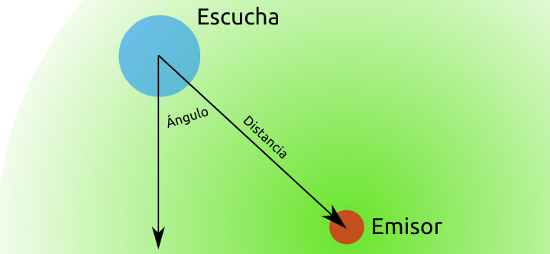
\includegraphics[scale=1]{img/audio3d-esquema.png}
    \end{center}
    
    Sistema liberado en un paquete independiente.
    
\end{frame}

    % Exportación de modelos 3D
    
\begin{frame}{Exportación de modelos 3D}
    
    \begin{center}
	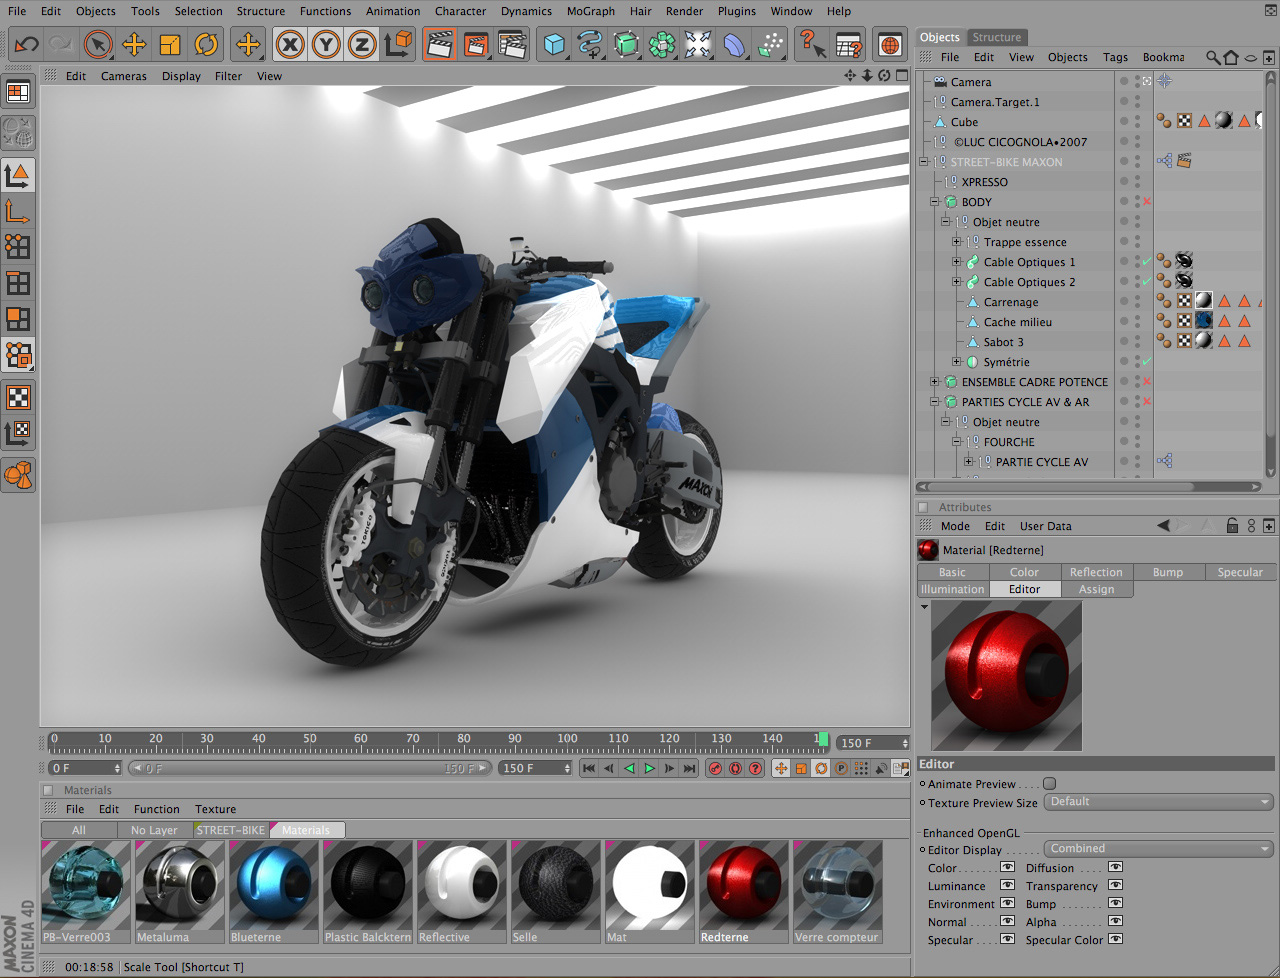
\includegraphics[scale=0.13]{img/cinema4d-moto.jpg}
    \end{center}
    
    \begin{alertblock}{Problema}
	\begin{itemize}
	    \item \textsc{Ogre3D} utiliza un formato propio para modelos y esqueletos.
	    \item El artista 3D trabaja con \textit{Cinema4D}.
	    \item El plugin de exportación no aplicaba escalas.
	\end{itemize}
    \end{alertblock}
\end{frame}


\begin{frame}{Exportación de modelos 3D}

    \begin{center}
	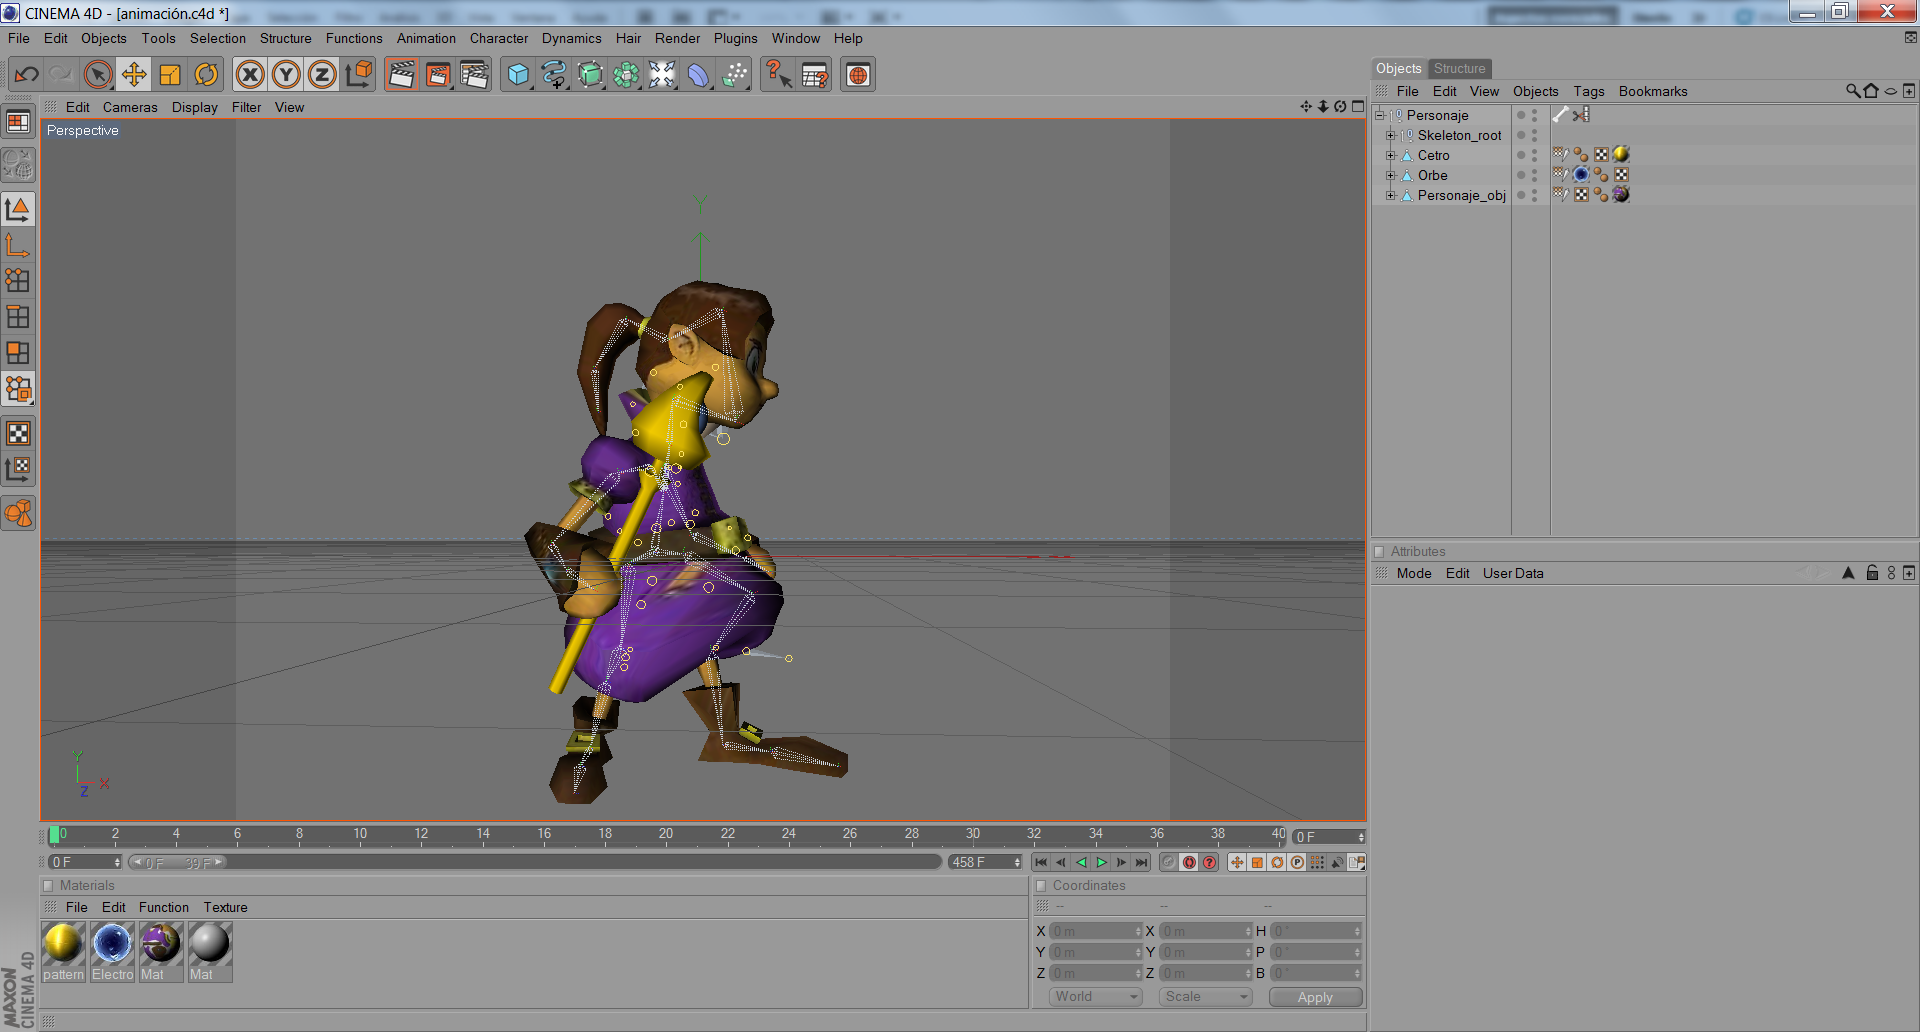
\includegraphics[scale=0.13]{img/cinema4d-personaje.png}
    \end{center}

    \begin{block}{Solución}
	\begin{itemize}
	    \item Script en Python.
	    \item Corrige escalas en mallas 3D y esqueletos.
	    \item Todos los elementos se ven a la misma escala.
	\end{itemize}
    \end{block}
\end{frame}
    
    % Carga de escenarios desde Blender
    
\begin{frame}{Creación de escenarios}

Desacoplar datos de código.

    \begin{alertblock}{Problema}
	\begin{itemize}
	    \item Necesidad de un editor de niveles.
	    \item Dificultad de crear un editor propio en 3D.
	    \item Información:
	    \begin{itemize}
		\item Escenario: objetos colisionables.
		\item Enemigos
		\item Música
		\item ...
	    \end{itemize}
	    \item Sistema sencillo: sin saber programar.
	\end{itemize}
    \end{alertblock}
\end{frame}

\begin{frame}{Creación de escenarios}
    
    \begin{center}
	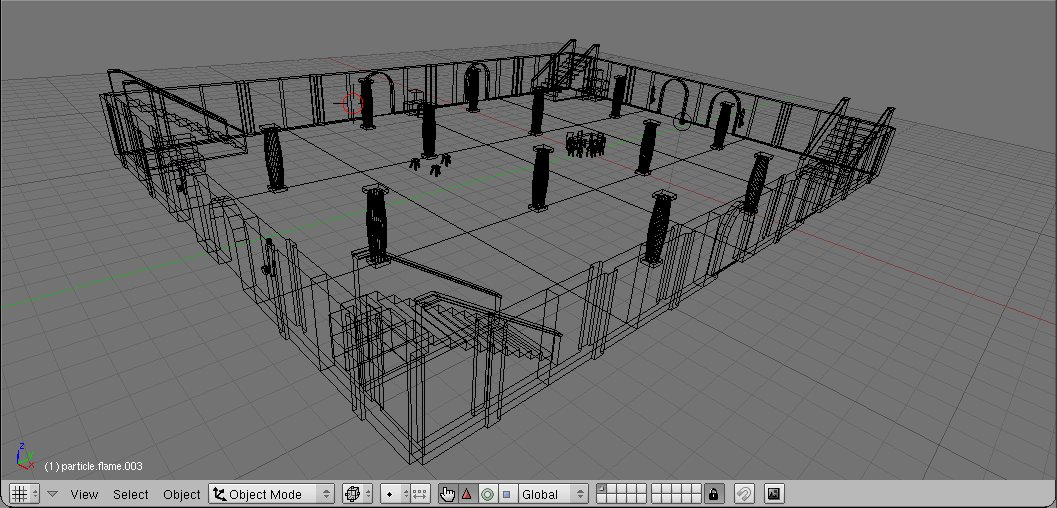
\includegraphics[scale=0.25]{img/blender-5.jpg}
    \end{center}
    
    \begin{block}{Solución}
	\begin{itemize}
	    \item Uso de Blender como editor de niveles.
	    \item Exportación de la escena a XML.
	    \item Carga del nivel en tiempo de ejecución.
	\end{itemize}
    \end{block}
\end{frame}

    % Detección de colisiones
    
\begin{frame}{Detección de colisiones}
    
    \begin{alertblock}{Problema}
	\begin{itemize}
	    \item Detectar colisiones entre elementos de juego.
	    \item Alto rendimiento.
	    \item Filtrado de colisiones.
	    \item Callbacks: métodos a llamar cuando se produzca una colisión.
	\end{itemize}
    \end{alertblock}
\end{frame}

\begin{frame}{Detección de colisiones}
    
    \begin{center}
	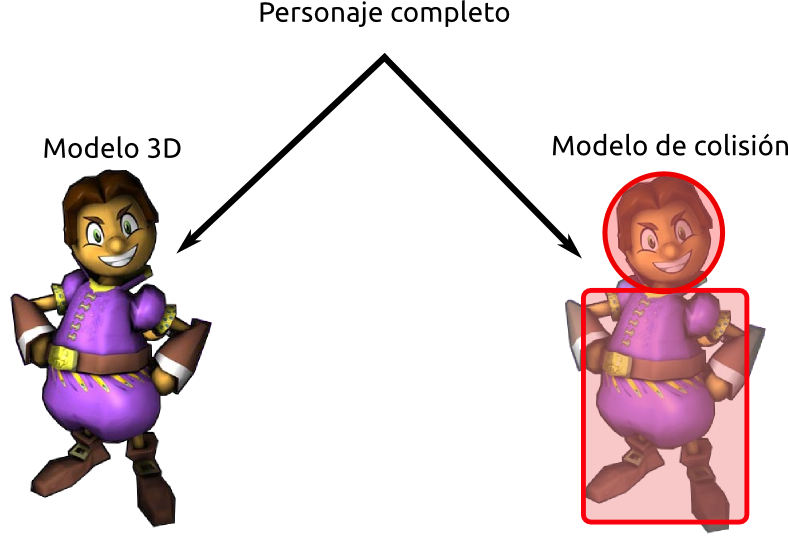
\includegraphics[scale=0.6]{img/colisiones.png}
    \end{center}
\end{frame}

\begin{frame}{Detección de colisiones}

    \begin{block}{Solución}
	\begin{itemize}
	    \item Jerarquía ampliable de formas geométricas.
	    \item Tests de colisión entre formas geométricas.
	    \item Polimorfismo dinámico.
	    \item Cuerpos formados por varias formas para mayor precisión.
	    \item Objetos de juego con un tipo para el filtrado.
	    \item Callbacks de comienzo, duración y final.
	\end{itemize}
    \end{block}
    
\end{frame}

\begin{frame}{Detección de colisiones}
    
    \begin{center}
	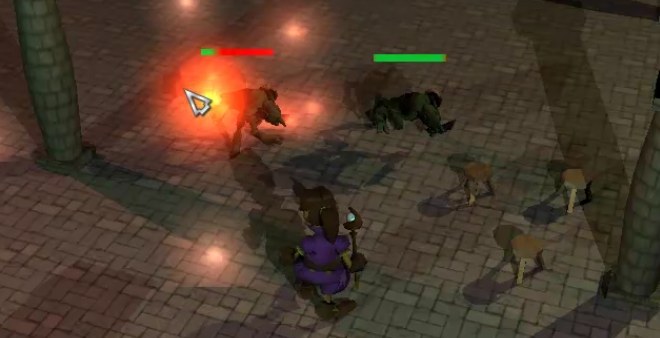
\includegraphics[scale=0.45]{img/siontower-colisiones.png}
    \end{center}
    
    Sistema liberado en un paquete independiente.
    
\end{frame}
    
    % Búsqueda de caminos
    
\begin{frame}{Búsqueda de caminos}
    
    \begin{alertblock}{Problema}
	\begin{itemize}
	    \item Los enemigos deben encontrar el camino hacia el personaje.
	    \item Existen obstáculos.
	    \item Necesidad de un sistema general (creación de niveles).
	    \item Eficiencia.
	\end{itemize}
    \end{alertblock}
    
    \begin{block}{Solución}
	\begin{itemize}
	    \item Malla de navegación diseñada con Blender.
	    \item Conversión de la malla en un grafo.
	    \item Algoritmo de Floyd.
	    \item Precomputación de caminos.
	\end{itemize}
    \end{block}
\end{frame}

\begin{frame}{Búsqueda de caminos}
    
    \begin{center}
	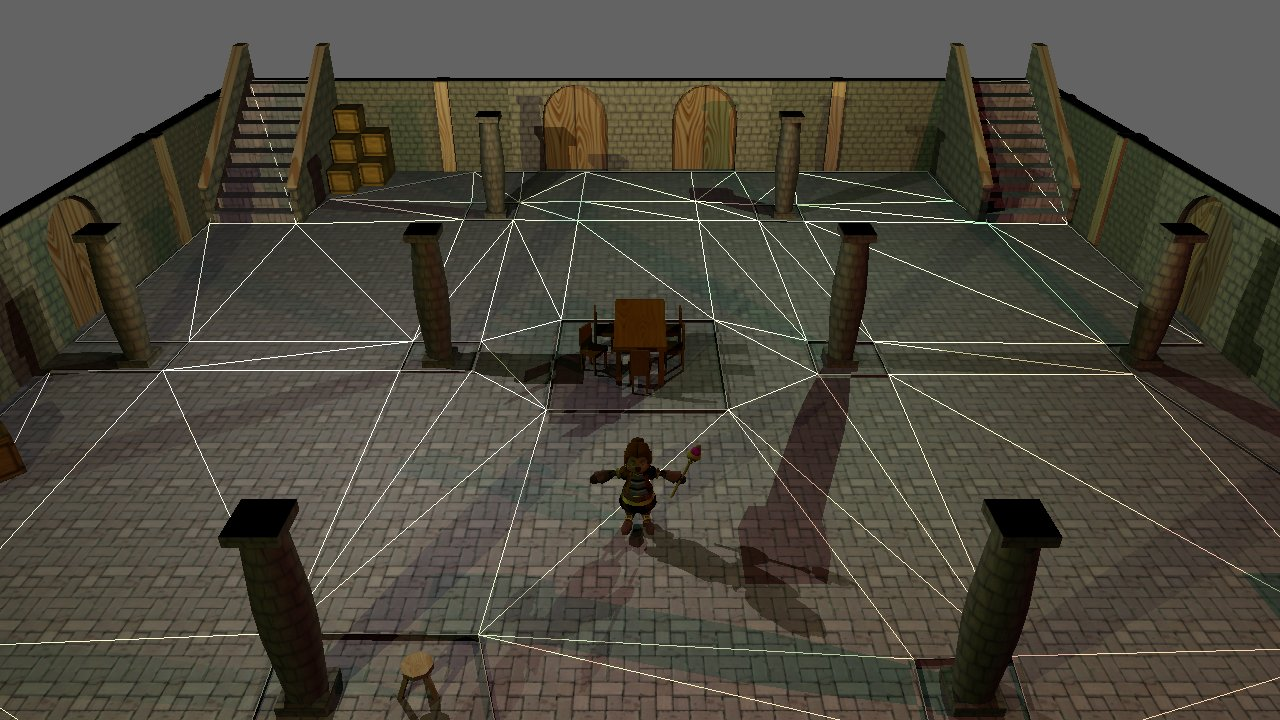
\includegraphics[scale=0.23]{img/siontower-navmesh.jpg}
    \end{center}
    
\end{frame}
    
    % Steering Behaviors
    
\begin{frame}{Steering Behaviors}
    
    \begin{alertblock}{Problema}
	\begin{itemize}
	    \item Enemigos siguen una línea de puntos.
	    \item No pueden colisionar entre ellos.
	    \item Deben moverse de forma suave.
	    \item No demasiada dificultad.
	\end{itemize}
    \end{alertblock}
    
    \begin{block}{Solución}
	\begin{itemize}
	    \item Algoritmos de movimiento dinámicos.
	    \item Fuerzas y aceleraciones.
	    \item Tienen en cuenta el personaje y el entorno.
	\end{itemize}
    \end{block}
\end{frame}
    
    % Versión publicada
    
\begin{frame}{Distribución}
    
    Hasta el momento se han publicado dos versiones de \textbf{Sion Tower}

    \begin{block}{Versiones}
	\begin{itemize}
	    \item Sion Tower 0.1 (demo técnica): 18-03-2011
	    \begin{itemize}
		\item Windows: 129 descargas.
		\item Fuentes y GNU/Linux: 90 descargas.
	    \end{itemize}
	    \item Sion Tower 1.0: 31-08-2011
	    \begin{itemize}
		\item Windows: 32 descargas
		\item Fuentes y GNU/Linux: 12 descargas.
	    \end{itemize}
	\end{itemize}
    \end{block}
\end{frame}
    
    % Documentación
    
\begin{frame}{Documentación}
    
    \begin{itemize}
	\item Blog de desarrollo
	
	\url{http://siondream.com/blog/category/pfc}\\
	
	\item Artículo en IberOgre
	
	\url{http://wikis.uca.es/iberogre/index.php/Sion_Tower}\\
	
	\item Doxygen
	
	\url{http://siondream.com/siontower-doxygen}\\
    \end{itemize}
\end{frame}

% Software utilizado
\section[Software]{Software utilizado}

\begin{frame}{Lenguajes y bibliotecas}
    \begin{block}{Lenguajes}
	\begin{itemize}
	    \item \textbf{C++}: código.
	    \item \textbf{Python}: herramientas auxiliares.
	    \item \textbf{XML}: datos (niveles, perfiles, interfaz).
	\end{itemize}
    \end{block}
    
    \begin{block}{Bibliotecas}
	\begin{itemize}
	    \item \textbf{Ogre3D}: motor de renderizado. 
	    \item \textbf{MyGUI}: complemento de \textsc{Ogre3D} para crear
	    interfaces.
	    \item \textbf{libSDL mixer}: efectos de sonido y pistas musicales.
	    \item \textbf{pugixml}: procesar ficheros XML.
	    \item \textbf{Boost}: extensión del lenguaje C++ similar a la \textsc{STL}.
	\end{itemize}
    \end{block}
\end{frame}

\begin{frame}{Herramientas}
    \begin{columns}[t]
	
	\column{150pt}
    
	\begin{itemize}
	    \item Subversion
	    \item GCC
	    \item Make
	    \item Vim
	    \item GNU Debugger
	    \item Valgrind
	    \item \LaTeX
	    \item Doxygen
	    \item Blender
	    \item GIMP
	\end{itemize}
	
	\column{150pt}
	
	\begin{itemize}
	    \item Inkscape
	    \item MyGUI Layout Editor
	    \item Particle Editor
	    \item Audacity
	    \item XvidCap
	    \item OpenShot
	    \item Planner
	    \item BOUML
	    \item Dia
	\end{itemize}
    \end{columns}
\end{frame}

% Comunidad y difusión
\section[Comunidad]{Comunidad y difusión}

\begin{frame}{Comunidad}

    \begin{center}
	
\includegraphics[scale=0.4]{img/enlaces.png}
    \end{center}

    \begin{block}{Difusión y contacto con la comunidad}
	\begin{itemize}
	    \item \textbf{Blog}: 70 artículos y 85.000 visitas.
	    \item \textbf{Forja}: 1.200 descargas.
	    \item \textbf{Twitter}: 100 seguidores.
	    \item \textbf{Web forja}: enlaces a otros medios.
	    \item \textbf{Youtube}: 10 vídeos con más de 2.800 reproducciones.
	\end{itemize}
    \end{block}
\end{frame}

\begin{frame}{V Concurso Universitario de Software Libre}

    \begin{center}
	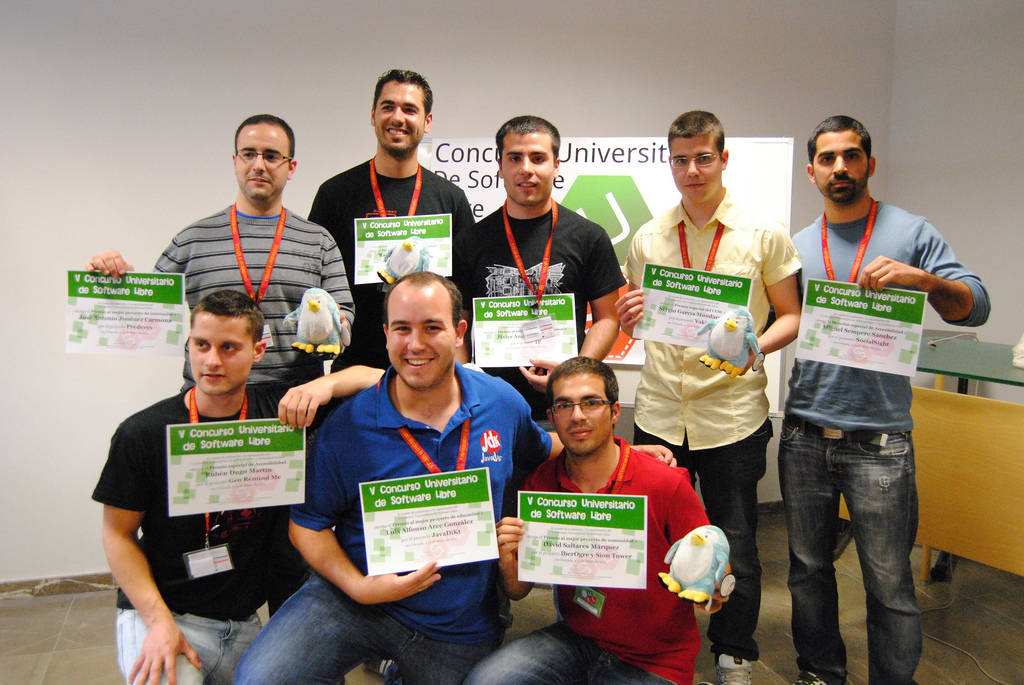
\includegraphics[scale=0.28]{img/vcusl.jpg}
    \end{center}

    \begin{block}{V CUSL}
	\begin{itemize}
	    \item 115 proyectos
	    \item \textbf{Premio nacional}: mejor proyecto de Comunidad.
	\end{itemize}
    \end{block}
\end{frame}

\begin{frame}{Difusión}

    \begin{block}{Apariciones en medios}
	\begin{itemize}
	\item Comunidades de desarrollo hispanohablantes.
	\item Prensa escrita: Diario de Cádiz, La Voz, Viva Cádiz, etc.
	\item Web oficial de \textsc{Ogre3D}.
	\item Proyecto recomendado por Steve Streeting, creador de \textsc{Ogre3D}.
	\end{itemize}
    \end{block}
\end{frame}

% Conclusiones
\section{Conclusiones}

\begin{frame}{Conclusiones personales}
    \begin{block}{Personales}
	\begin{itemize}
	    \item Videojuegos en 3D
	    \item Bibliotecas
	    \item Matemáticas
	    \item Lenguajes: C++ y Python
	    \item Optimización
	    \item Técnicas de IA
	    \item Trabajo en equipo
	    \item Redacción en MediaWiki
	    \item Trabajo en wikis
	\end{itemize}
    \end{block}
\end{frame}


\begin{frame}{Conclusiones técnicas}
    \begin{columns}[t]
    \column{150pt}
    \begin{block}{IberOgre}
	\begin{itemize}
	    \item Bloques.
	    \item Dificultad ascendente.
	    \item Conceptos de matemáticas.
	    \item Subsistemas de \textsc{Ogre3D}.
	    \item Tecnologías complementarias.
	\end{itemize}
    \end{block}
    \column{150pt}
    \begin{block}{Sion Tower}
	\begin{itemize}
	    \item Multiplataforma
	    \item Cuatro niveles, tres enemigos y tres hechizos.
	    \item Iluminación y sombras dinámicas.
	    \item Sistemas de partículas.
	    \item Alto rendimiento.
	    \item Ampliable con Blender.
	    \item Internacionalizado.
	\end{itemize}
    \end{block}
    \end{columns}
\end{frame}

\begin{frame}{Posibles mejoras}
    \begin{block}{IberOgre}
	\begin{itemize}
	    \item Consolidación de la comunidad.
	    \item Artículos sobre videojuegos.
	    \item Subsistema de \textit{shading}.
	    \item Juego en red.
	\end{itemize}
    \end{block}
    
    \begin{block}{Sion Tower}
	\begin{itemize}
	    \item Nuevos hechizos y enemigos.
	    \item Niveles de mayor tamaño.
	    \item Escenas narrativas animadas.
	\end{itemize}
    \end{block}
\end{frame}



\begin{frame}{Estadísticas de la forja}
    
    \begin{center}
	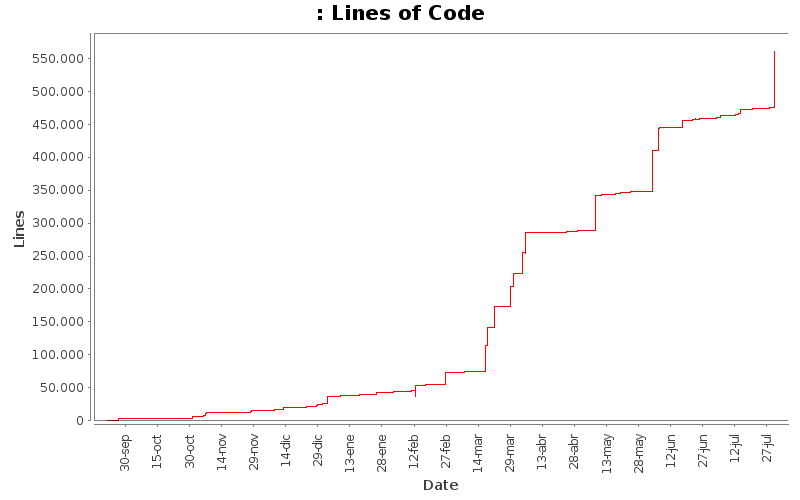
\includegraphics[scale=0.25]{img/loc.png}
    \end{center}
    
    \begin{block}{Cifras}
	\begin{itemize}
	    \item 550 revisiones.
	    \item 21.193 líneas de código (\textit{trunk}).
	    \item \url{http://siondream.com/iberogre-siontower-statsvn}
	\end{itemize}
    \end{block}
\end{frame}

    % Estadísticas
    
\begin{frame}
    \frametitle{Estadísticas wiki}

    \begin{columns}[t]
    \column{150pt}
        
	\begin{block}{Datos}
            \begin{itemize}
		\item \textbf{Artículos publicados}: 27
                \item \textbf{Páginas en PDF}: 400
		\item \textbf{Ediciones}: 698
		\item \textbf{Usuarios}: 22
		\item \textbf{Visitas}: 33.538
            \end{itemize}            
        \end{block}

    \column{150pt}

	\begin{center}
	    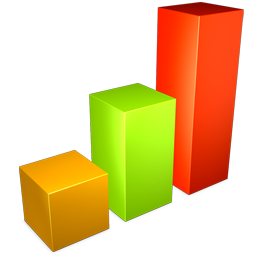
\includegraphics[scale=0.25]{img/estadisticas.png}
	\end{center}

    \end{columns} 

\end{frame}

\section{Bibliografía}
\begin{frame}{Bibliografía}
    \begin{thebibliography}{4}
    \small{
	\bibitem{eric05}
	Christer Ericson
	\emph{Real Time Collision Detection}
	Morgan Kaufmann
	2005
	
	\bibitem{greg09}
	Jason Gregory
	\emph{Game Engine Architecture}
	Peters Ltd.
	2009
	
	\bibitem{Erich Gammma}
	\emph{Design Patterns}
	Addison Wesley
	1994
	
	\bibitem{mill09}
	Ian Millington y John Fudge
	\emph{Artificial Intelligence for Games}
	Morgan Kaufmann
	2009
	
	\bibitem{hess09}
	Roland Hess
	\emph{The Essential Blender}
	Blender Foundation
	2009
	
	\bibitem{larm02}
	Craig Larman
	\emph{Applying UML and Patterns}
	Prentice Hall
	2002
	
	\bibitem{pilgr04}
	Mark Pilgrim
	\emph{Dive Into Python}
	Apress
	2004
	
	\bibitem{gera09}
	Gerardo Aburruzaga García, Inmaculada Medina Bulo y Francisco Palomo Lozano
	\emph{Fundamentos de C++}
	Servicio de Publicaciones de la UCA
	2009
    }
    \end{thebibliography}
\end{frame}

\begin{frame}[fragile]
\transdissolve
    \frametitle{}
    
    \begin{center}
	\textbf{Gracias por su atención}\\
	
	\vspace*{0.5cm}
	
	En primer lugar vamos a hacer una demostración...

	\vspace*{0.7cm}
	
	\pause

	\Huge{\textbf{¿Preguntas?}}
	
	\vspace*{0.7cm}
	
	\small{
	\begin{verbatim}
	      https://forja.rediris.es/projects/cusl5-iberogre
	\end{verbatim}
	}
    \end{center}
\end{frame}


\licencia

\end{document}
